% Vertx Instalation process
%
% External sources
%

\newpage
\section*{Instalación del gestor de documentos Mongo}
	\paragraph{Para sistemas basados en Ubuntu (12.04).}
	\paragraph{Es necesario agregar la llave de los servidores que tienen las fuentes de mongo a las llaves del sistema actual, eso se realiza mediante el siguiente comando:}
	\begin{alltt}
		sudo apt-key adv --keyserver hkp://keyserver.ubuntu.com:80 --recv 7F0CEB10
	\end{alltt}
	\paragraph{Después se procede a agregar los servidores de Mongo a la lista de distribución y actualizar los paquetes del sistema.}
	\begin{alltt}
		echo "deb http://repo.mongodb.org/apt/ubuntu precise/mongodb-org/3.0 multiverse" 
		| sudo tee /etc/apt/sources.list.d/mongodb-org-3.0.list

		sudo apt-get update
	\end{alltt}
	\paragraph{Finalmente se procede a la instalación de mongo, eso se hace mediante la siguiente línea en la terminal.}
	\begin{alltt}
		sudo apt-get install -y mongodb-org
	\end{alltt}
	\paragraph{Al finalizar la instalación, se puede acceder al gestor mediante la siguiente línea}
	\begin{alltt}
		mongo
	\end{alltt}
	\paragraph{Mostrando finalmente el acceso al gestor como lo muestra la siguiente imagen.}
	\begin{figure}[h!]
    	\centering
    		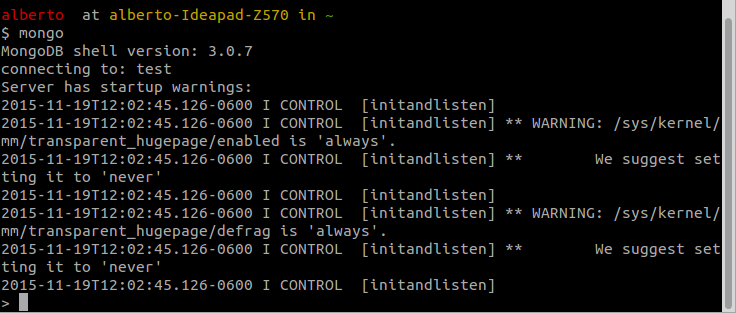
\includegraphics[width=\textwidth]{./images/TerminalMongo}
    		\caption{Captura del gestor de documentos Mongo.}
  	\end{figure}
  \paragraph{Ahora es necesario realizar la creación de la base de tipo Places (Fast Eagle), utilizando la siguiente línea en una terminal nueva.}
  \begin{alltt}
    mongoimport --db=Ambienta2MX-Places --jsonArray --collection=Places -v placesdb.json
  \end{alltt}
  \paragraph{El archivo placesdb.json se encuentra dentro del disco del proyecto.}
  \paragraph{Para poder utilizar los índices geográficos de mongo es necesario crearlos, para ello es necesario crear las bases de tipo MX en el servidor o servidores deseados y generar un índice de la siguiente forma.}
  \begin{alltt}
    db.<DesiredCollection>.createIndex( { <LocationField> : "2dsphere" } )
  \end{alltt}
  \paragraph{Cambiando los valores de ``DesiredCollection'' y ``LocationField'' por los valores en las colecciones de Places, Weather o Pollution en el primero y location en el último.}
\addcontentsline{toc}{chapter}{Anexo 4: Instalación de Mongo} 